\section{Agile Manifesto}
This section highlights the most important principles of the Agile
Manifesto.

{\bf Individuals and interactions} \emph{over processes and
tools.}\cite{AgileManifesto} Developing software is an intellectual and creative
process, which is challenging and spectacularly complicated. Managers do not
make any differentiation between a software developer and a house builder. They
assume they can plug and play people into a software project as they can in the
house building industry, which is obviously not the same thing. Agile teams are
most commonly compared to sports teams, which can only win if the team members
play together. Teamwork requires by definition a great deal of communication
skills. Processes are important, but not vital. If you had a choice between an
NBA level basketball team and a group of very smart, athletic and toll people
who never heard of basketball before, but got it explained in detail just prior
to the match, on which team would you bet your money on? And always remember,
that although tools are helpful a fool with a tool is still a fool.

{\bf Working software} \emph{over comprehensive
documentation.}\cite{AgileManifesto} The goal of software development is
software, not documentation, otherwise it would be called documentation
development.\cite{Ambler200204} Documentation is important, but not a priority.
And why should it be? If you think about it, working software is even more
explanatory than a technical, gibberish document.

{\bf Customer collaboration} \emph{over contract
negotiation.}\cite{AgileManifesto} Developing software is a creative process and
the fact that software developers are the only stakeholders in the software
project is nothing more than an illusion. The customer \emph{develops} ideas and
the software developer implements them. Thus the customer becomes a vital part
of the team and communication skills are required yet again. The customer has to
be creative himself. Since creativity is an iterative process, there is just no
way, the customer could communicate his wishes to the software developer
upfront. And even if he could, would the software developer go ahead and build
the whole system in one sit?

{\bf Responding to change} \emph{over following a plan.}\cite{AgileManifesto}
The fact that change {\bf is} the state in the software world is undeniable.
Technology, business environment, skills, domain understanding change over time
and there is nothing you can do about it. In fact you should embrace change and
act now instead of planning for tomorrow to paraphrase the surprisingly
effective way of thinking: \enquote{Implement for today, design for
tomorrow.}\cite{BeckAndres200411}

\section{Extreme Programming}
This section introduces XP and explains the origins of the \emph{extreme}
part in its naming.

The main purpose of XP is to reduce project risk, making everyone happy on its
way. The programmers work on tasks that really matter. These tasks bring joy and
joy is the reason why they got into programming in the first place. In
addition to that, they never have to make important decisions on their own and
therefore become fearless of change. The customers and managers receive rapid
feedback, which gives them the ability to steer the project in the right
direction or even entirely change the course of action.\cite{BeckAndres200411}

XP maximizes agile principles and practices buy boosting them to extreme levels
and this is where the name comes from:
\begin{itemize}
\item If code reviews are good, we'll review code all the time (pair
programming).
\item If testing is good, everybody will test all the time (unit testing), even
the customers (functional testing).
\item If design is good, we'll make it part of everybody's daily business
(refactoring).
\item If simplicity is good, we'll always leave the system with the simplest
design that supports its current functionality (the simplest thing that could
possibly work).
\item If architecture is important, everybody will work defining and refining
the architecture all the time (metaphor).
\item If integration testing is important, then we'll integrate and test
several times a day (continuous integration).
\item If short iterations are good, we'll make the iterations really, really
short - seconds and minutes and hours, not weeks and months and years (the
Planning Game).\cite{BeckAndres200411}
\end{itemize}

\section{Agile Modeling}
This section introduces AM and explains its goals, but before jumping into AM we
discuss why bother with modeling at all.

Models are artifacts, which help you understand what you are building or aid the
communication with your team. And since communication is so important to an
agile team (or any team for that matter), modeling is also important.

\subsection{What is AM?}
AM is not a complete software process like XP. Instead AM is a modification for
a software process as presented in the following figure.
 \begin{figure}[h]
  \caption[AM Scope]{AM Scope\cite{AM}}
  \label{jee}
  \center
  	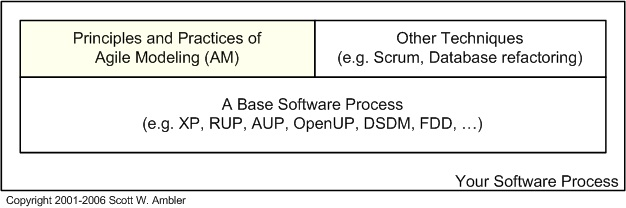
\includegraphics[scale=0.5]{../resources/amScope.jpg}
\end{figure}
AM is all about modeling and documentation. AM does not show how to create new
models, but how to apply existing modeling techniques. Am values content over
representation. AM
\begin{itemize}
\item is an attitude, not a prescriptive process
\item is a supplement to existing methods; not a complete methodology
\item is complementary to other modeling processes
\item is a way to work together effectively to meet the needs of project
stakeholders
\item is effective and is about being effective
\item is something that works in practice; isn't an academic theory
\item is not a silver bullet
\item is for the average developer, but is not a replacement for competent
people
\item is not an attack on documentation
\item is not an attack on CASE tools\cite{Ambler200204}
\end{itemize}

\subsection{What makes models agile?}
AM does not take the model driven approach. The audience for models are people,
not computers. Therefore neither models on top of models nor a
perfect specification is required. So what is an agile model? \enquote{An agile
model is a model that is just barely good enough.}\cite{Ambler200204} It does
not even have to be graphical. The following list helps you to determine whether
your model is good enough.
\begin{description}
\item {\bf Agile models fulfill their purpose.} Examples for purposes include:
communicating the scope of your effort to a stakeholder or understanding
architecture or design of a part of an application.
\item {\bf Agile models are understandable.} The notation of your model should
conform to the skills and expertise of your audience.
\item {\bf Agile models are sufficiently accurate.} An imperfect model is better
than a non-existent one. If the navigation system in your car misses a street you
have a choice to either update the map or to ignore this fact if you never drive
nowhere near that street anyway. But you would never throw your navigation
system away because of it or would you?
\item {\bf Agile models are sufficiently consistent.} The audience for models
are people. The world is not going to come to an end if you use a dotted arrow
instead of the continuous one in your UML class diagram.
\item {\bf Agile models are sufficiently detailed.} The level of detail should
be chosen carefully. Remember, \emph{just good enough} is perfect for an agile
model.
\item {\bf Agile models provide positive value.} This one is very important. If
you do not know why you are creating a model or the person who requested it could
not explain why he needed it, than you probably should not bother modeling. It
is a business after all. Everything you do should add positive value to the
project.
\item {\bf Agile models are as simple as possible.} Many factors contribute to
complexity of a model. Among them are: the level of detail or
the comprehensiveness of the notation.
\end{description}

\subsection{What makes documentation agile?}
The fact, that agile developers produce as less documentation as possible is
very far from the truth. Yes, agile folks travel light, which means that not
every document is made persistent and maintained until the end of all eternity.
But this also means that being agile means manufacturing even more documentation
as you would do when following any other methodology. Documentation is a very
important part of any system, which has to be maintained for a given period of
time and agile developers realize that fact.

So when is a document agile?
\begin{description}
\item {\bf Agile documents maximize stakeholder investment.} Although
documentation is important it has a very low priority in an agile software
development process. This means, that if there is an alternative, which would
provide more value to the project, than you should choose it over documentation.
Use the best tool for the job. Examples of alternatives include: cleaning the
code or communicating face to face instead of writing emails and documenting
every single design decision.
\item {\bf Agile documents are \enquote{lean and mean}.} \enquote{An agile
document contains just enough information to fulfill its purpose.}\cite{Ambler200204} Agile modelers value
content over representation. If you are writing a document in prose and need to
add a diagram to it, consider a handwritten document over a perfectly generated
colored artifact produced by a Computer-Aided Software Engineering (CASE) tool.
\item {\bf Agile documents fulfill a purpose.} As with models, you always need
a very good reason for creating a document. Make sure, that every second you
invest in creating a document is worth it.
\item {\bf Agile documents describe information that is less likely to change.}
Things that change a lot are hard to document and make any documentation effort
unmaintainable. Chances are, you do not need such a document at all.
\item {\bf Agile documents describe \enquote{good things to know}.} The
information in an agile document requires a right to exist. Perfect candidates are: the
reasoning behind a design decision, usage procedures or operational procedures.
\item {\bf Agile documents have a specific customer and facilitate the work
efforts of that customer.} Know your audience, even if your audience is you.
Consider different types of documents, which are suited best for the job.
\item {\bf Agile documents are sufficiently accurate, consistent, and detailed.}
\enquote{Agile documents do not need to be perfect, they just need to be good
enough.}\cite{Ambler200204}
\item {\bf Agile documents are sufficiently indexed.} Time is money. You cannot
afford looking over 2000 pages Software Architecture Document (SAD) to find out
which signature a certain method has. \enquote{Your indexing scheme
should reflect the needs of a document's audience.}\cite{Ambler200204}
\end{description}
Being an agile modeler is not an excuse for creating sloppy documentation.
Sometimes documentation needs to be perfect. Always remember the purpose of the
documentation you are creating and be aware of your audience.

\section{AM \& XP}
Although AM can be tailored to any software process, it was not only designed
for but is also based on XP. 
\subsection{Values}
XP follows a simple set of values:
\begin{description}
  \item {\bf communication} - Most problems in any project can be traced back to
  someone not talking to someone else about something important.
  \item {\bf simplicity} - Simple and easy are two different concepts. As
  developer you are confronted with complexity on a day to day basis creating
  things, which are easy to use for others. Being easy to use does not mean that
  the thing you are using is simple. In fact it is quite the opposite.
  \enquote{XP is making a bet. It is betting that it is better to do a simple
  thing today and pay a little more tomorrow to change it if it needs it, than to do a more
  complicated thing today that may never be used anyway.}\cite{BeckAndres200411}
  \item {\bf feedback} - \enquote{Concrete feedback about
the current state of the system is absolutely priceless.}\cite{BeckAndres200411}
The more you have, the better.
  \item {\bf courage} - Courage is the most intriguing one. You should not be
  afraid of trying out new things, throwing code away, throwing design decisions
  away after trying them out, doing major refactoring if they need to be made.
  Courage by itself would not make much sense, but combined with communication,
  simplicity and feedback, courage gives you a major boost comparable to
  the nitrous oxide injection of a car.
\end{description}
AM adopts all theses values and adds another one - \emph{humility}.
\subsection{Principles}
XP has principles, which are more concrete, than the high-level values.
\begin{itemize}
  \item Rapid feedback
  \item Assume simplicity
  \item Incremental change
  \item Embracing change
  \item Quality work\cite{BeckAndres200411}
\end{itemize}
AM adopts most of those and adds few of its own.
\begin{itemize}
  \item Software is your primary goal
  \item Enabling the next effort is your secondary goal
  \item Travel light
  \item Assume simplicity
  \item Embrace change
  \item Incremental change
  \item Model with a purpose
  \item Multiple models
  \item Quality work
  \item Maximize stakeholder investment\cite{Ambler200204}
\end{itemize}
\subsection{Practices}
Here are all XP practices:
\begin{description}
  \item {\bf The Planning Game} Quickly determine the scope of the next  
  release by combining business priorities and technical estimates. As reality
  overtakes the plan, update the plan.
  \item {\bf Small releases} Put a simple system into production quickly, then
  release new versions on a very short cycle.
  \item {\bf Metaphor} Guide all development with a simple shared story of how
  the whole system works.
  \item {\bf Simple design} The system should be designed as simply as possible
  at any given moment. Extra complexity is removed as soon as it is discovered.
  \item {\bf Testing} Programmers continually write unit tests, which must run
  flawlessly for development to continue. Customers write tests demonstrating
  that features are finished.
  \item {\bf Refactoring} Programmers restructure the system without changing
  its behavior to remove duplication, improve communication, simplify, or add
flexibility.
  \item {\bf Pair programming} All production code is written with two
  programmers at one machine.
  \item {\bf Collective ownership} Anyone can change any code anywhere in the
  system at any time.
  \item {\bf Continuous integration} Integrate and build the system many times
  a day, every time a task is completed.
  \item {\bf 40 hour week} Work no more than 40 hours a week as a rule. Never
  work overtime a second week in a row.
  \item {\bf On-cite customer} Include a real, live user on the team, available
  full-time to answer questions.
  \item {\bf Coding standards} Programmers write all code in accordance with
  rules emphasizing communication through the code.\cite{BeckAndres200411}
\end{description}
AM practices are categorized into four groups:
\begin{enumerate}
  \item Iterative and incremental approach to modeling:
	  \begin{description}
	  \item {\bf Apply the Right Artifact(s)}
	  \item {\bf Create Several Models in Parallel}
	  \item {\bf Iterate to Another Artifact}
	  \item {\bf Model in Small Increments}
	  \end{description}
  \item Effective teamwork and communication within your team and with your
  project stakeholders:
  	  \begin{description}
	  \item {\bf Model with Others}
	  \item {\bf Active Stakeholder Participation}
	  \item {\bf Collective Ownership}
	  \item {\bf Display Models Publicly}
	  \end{description}
  \item Enabling simplicity within your modeling efforts:
  	  \begin{description}
	  \item {\bf Create simple content}
	  \item {\bf Depict models simply}
	  \item {\bf Use the simplest tools}
	  \end{description}
  \item Validation:
  	  \begin{description}
	  \item {\bf Consider Testability}
	  \item {\bf Prove it With Code}\cite{Ambler200204}
	  \end{description}
\end{enumerate}

\subsection{The potential fit between AM and XP}
In this section we compare how AM practices fit to XP.

{\bf Active Stakeholder Participation } is simply a new take on XP's
\emph{On-cite customer} practice. AM uses the term project stakeholder in place
of customer and focuses on the concept of their active participation, hence Active
Stakeholder Participation and not On-Site Stakeholder.

{\bf Apply Modeling Standards} is the AM version of XP's \emph{Coding Standards}
practice.

{\bf Apply Patterns Gently} reflects the You Ain't Gonna Need It (YAGNI)
principle to the effective application of patterns within your system, in
conformance to XP's practice of \emph{Simple Design}.

{\bf Apply the Right Artifact(s)} is not explicitly described by XP principles
and practices although is very much aligned with XP philosophies of
\emph{\enquote{if you need it do it}} and using the most appropriate tool or
technique for the job at hand.

{\bf Collective Ownership} has been directly transfered to AM.

{\bf Create Several Models in Parallel} is a modeling-specific practice. XP
developers can clearly work on several models - such as CRC cards, acceptance
test cases, and sketches - if they choose to do so.

{\bf Create Simple Content} is complementary XP's \emph{Simple Design} practice
that advises to keep your models as simple as possible.

{\bf Depict Models Simply} is complementary XP's \emph{Simple Design} practice
that suggests that your models do not need to be fancy to be effective, perfect
examples of which are CRC cards and user stories.

{\bf Discard Temporary Models} reflects XP's \emph{Travel Light} principle,
which AM has adopted, explicitly advising you to dispose of models that you no
longer need.

{\bf Display Models Publicly} reflects XP's (and AM's) value of
\emph{Communication}, principle of \emph{Open and Honest Communication} (adopted
by AM), and reflects its practice of \emph{Collective Ownership}.

{\bf Formalize Contract Models} is not currently reflected within
XP, well perhaps in its \enquote{if you need to then do it} philosophy. This
practice was included in AM to provide guidance for how to deal with the very
common situation of integrating with other systems.

{\bf Iterate to Another Artifact} explicitly states, in a general form, the
practice of XP developers to iterate between working on various artifacts such
as source code, CRC cards, and tests.

{\bf Model in Small Increments} his practice supports XP's iterative and
increment approach to development. Both XP and AM prefer an emergent approach
to development and not a big design up front (BDUF) approach.

{\bf Model With Others} is the AM version of XP's \emph{Pair Programming}
practice.

{\bf Prove it With Code} is the AM version of XP's \emph{Concrete Experiments}
principle. In fact, it was originally called Concrete Experiments although was
renamed when it was evolved into a practice.

{\bf Reuse Existing Resources} is not explicitly included in XP, although it
clearly isn't excluded either. XP developers are practical, if there is
something available that can be appropriately reused then they will likely
choose to do so.

{\bf Single Source Information} reflects the XP concept of \emph{traveling
light}.

{\bf Update Only When it Hurts} reflects AM and XP's \emph{Travel Light}
principle, advising that you should only update an artifact only when you
desperately need to.

{\bf Use the Simplest Tools} This practice reflects AM and XP's \emph{Assume
Simplicity} principle and is consistent with XP's preference for low-tech tools
such as index cards for modeling.\cite{AM}